\documentclass[sans,mathserif]{beamer}

\mode<presentation>
{
  \usetheme{Warsaw}
  % \usetheme{Madrid}
  % or ...

  %\setbeamercovered{transparent}
  % or whatever (possibly just delete it)
}

% \usepackage[czech]{babel}
\usepackage[utf8]{inputenc}

\usepackage{graphicx} % nezbytné pro standardní vkládání obrázků do dokumentu
\usepackage{multirow}

\usepackage{times}
\usepackage[T1]{fontenc}
% Or whatever. Note that the encoding and the font should match. If T1
% does not look nice, try deleting the line with the fontenc.

\usepackage[style=authoryear]{biblatex}
\usepackage{hyperref}
\usepackage{amssymb}

\setbeamertemplate{bibliography item}{%
  \ifboolexpr{ test {\ifentrytype{book}} or test {\ifentrytype{mvbook}}
    or test {\ifentrytype{collection}} or test {\ifentrytype{mvcollection}}
    or test {\ifentrytype{reference}} or test {\ifentrytype{mvreference}} }
    {\setbeamertemplate{bibliography item}[book]}
    {\ifentrytype{online}
       {\setbeamertemplate{bibliography item}[online]}
       {\setbeamertemplate{bibliography item}[article]}}%
  \usebeamertemplate{bibliography item}}

% \defbibenvironment{bibliography}
%   {\list{}
%      {\settowidth{\labelwidth}{\usebeamertemplate{bibliography item}}%
%       \setlength{\leftmargin}{\labelwidth}%
%       \setlength{\labelsep}{\biblabelsep}%
%       \addtolength{\leftmargin}{\labelsep}%
%       \setlength{\itemsep}{\bibitemsep}%
%       \setlength{\parsep}{\bibparsep}}}
%   {\endlist}
%   {\item}

% \addbibresource{bajer2013model.bib}
\bibliography{bajer2013model}

\newcommand{\xx}{\mathrm{\mathbf{x}}}
\newcommand{\XX}{\mathrm{\mathbf{X}}}
\newcommand{\yy}{\mathrm{\mathbf{y}}}
\newcommand{\ttheta}{\mathbf{\theta}}
\newcommand{\eell}{\boldsymbol\ell}
\newcommand{\R}{\mathrm{\mathbb{R}}}
\newcommand{\CC}{\mathrm{\mathbf{C}}}
\newcommand{\KK}{\mathrm{\mathbf{K}}}
\newcommand{\II}{\mathrm{\mathbf{I}}}
\newcommand{\uv}[1]{\quotedblbase #1\textquotedblleft}
\newcommand{\blue}[1]{{\color{blue} #1}}

\title[MGSO with Gaussian Processes for Black-Box Opt.
  \hspace{4em}\insertframenumber] % (optional, use only with long paper titles)
%   \hspace{2em}\insertframenumber/\inserttotalframenumber] % (optional, use only with long paper titles)
  {Model Guided Sampling Optimization with Gaussian Processes \\ for Expensive Black-Box Optimization}

\author[Luk\'{a}\v{s} Bajer, Viktor Charypar, Martin Hole\v{n}a]
{Luk\'{a}\v{s}~Bajer$^{1,2}$, Viktor Charypar$^3$, Martin Hole\v{n}a$^2$}
% - Give the names in the same order as the appear in the paper.
% - Use the \inst{?} command only if the authors have different
%   affiliation.

\institute[MFF UK, UI AVČR, FJFI ČVUT] % (optional, but mostly needed)
{
  $^1$Faculty of Mathematics and Physics, Charles University, \\
  $^2$Institute of Computer Science, Czech Academy of Sciences, and \\
  $^3$Faculty of Nuclear Sciences, Czech Technical University
\vskip 1em
  Prague, Czech Republic
}
% - Use the \inst command only if there are several affiliations.
% - Keep it simple, no one is interested in your street address.

\date{GECCO, Amsterdam, July 2013}
% \date[EvA 2008] % (optional, should be abbreviation of conference name)
% {AIL086 Evolutionary Algorithms 2}
% % - Either use conference name or its abbreviation.
% % - Not really informative to the audience, more for people (including
% %   yourself) who are reading the slides online

% \subject{Theoretical Computer Science}
% % This is only inserted into the PDF information catalog. Can be left
% % out.

% If you have a file called "university-logo-filename.xxx", where xxx
% is a graphic format that can be processed by latex or pdflatex,
% resp., then you can add a logo as follows:

% \pgfdeclareimage[height=0.5cm]{mff-logo}{img/mff-logo}
% \logo{\pgfuseimage{mff-logo}}


% Delete this, if you do not want the table of contents to pop up at
% the beginning of each subsection:
\AtBeginSection[]
{
  \begin{frame}<beamer>{Contents}
  \tableofcontents[currentsection,currentsubsection]
  \end{frame}
}
% \AtBeginSubsection[]
% {
%   \begin{frame}<beamer>{Contents}
%   \tableofcontents[currentsection,currentsubsection]
%   \end{frame}
% }


% If you wish to uncover everything in a step-wise fashion, uncomment
% the following command:

%\beamerdefaultoverlayspecification{<+->}


\begin{document}

\begin{frame}
  \titlepage
\end{frame}

\begin{frame}{Contents}
  \tableofcontents
  % You might wish to add the option [pausesections]
\end{frame}


% Structuring a talk is a difficult task and the following structure
% may not be suitable. Here are some rules that apply for this
% solution:

% - Exactly two or three sections (other than the summary).
% - At *most* three subsections per section.
% - Talk about 30s to 2min per frame. So there should be between about
%   15 and 30 frames, all told.

% - A conference audience is likely to know very little of what you
%   are going to talk about. So *simplify*!
% - In a 20min talk, getting the main ideas across is hard
%   enough. Leave out details, even if it means being less precise than
%   you think necessary.
% - If you omit details that are vital to the proof/implementation,
%   just say so once. Everybody will be happy with that.

\section{Optimization of empirical functions}

\begin{frame}
  \frametitle{Optimization of expensive black-box functions}
  \begin{itemize}[<+->]
    \item optimization of black-box functions
      \begin{figure}
      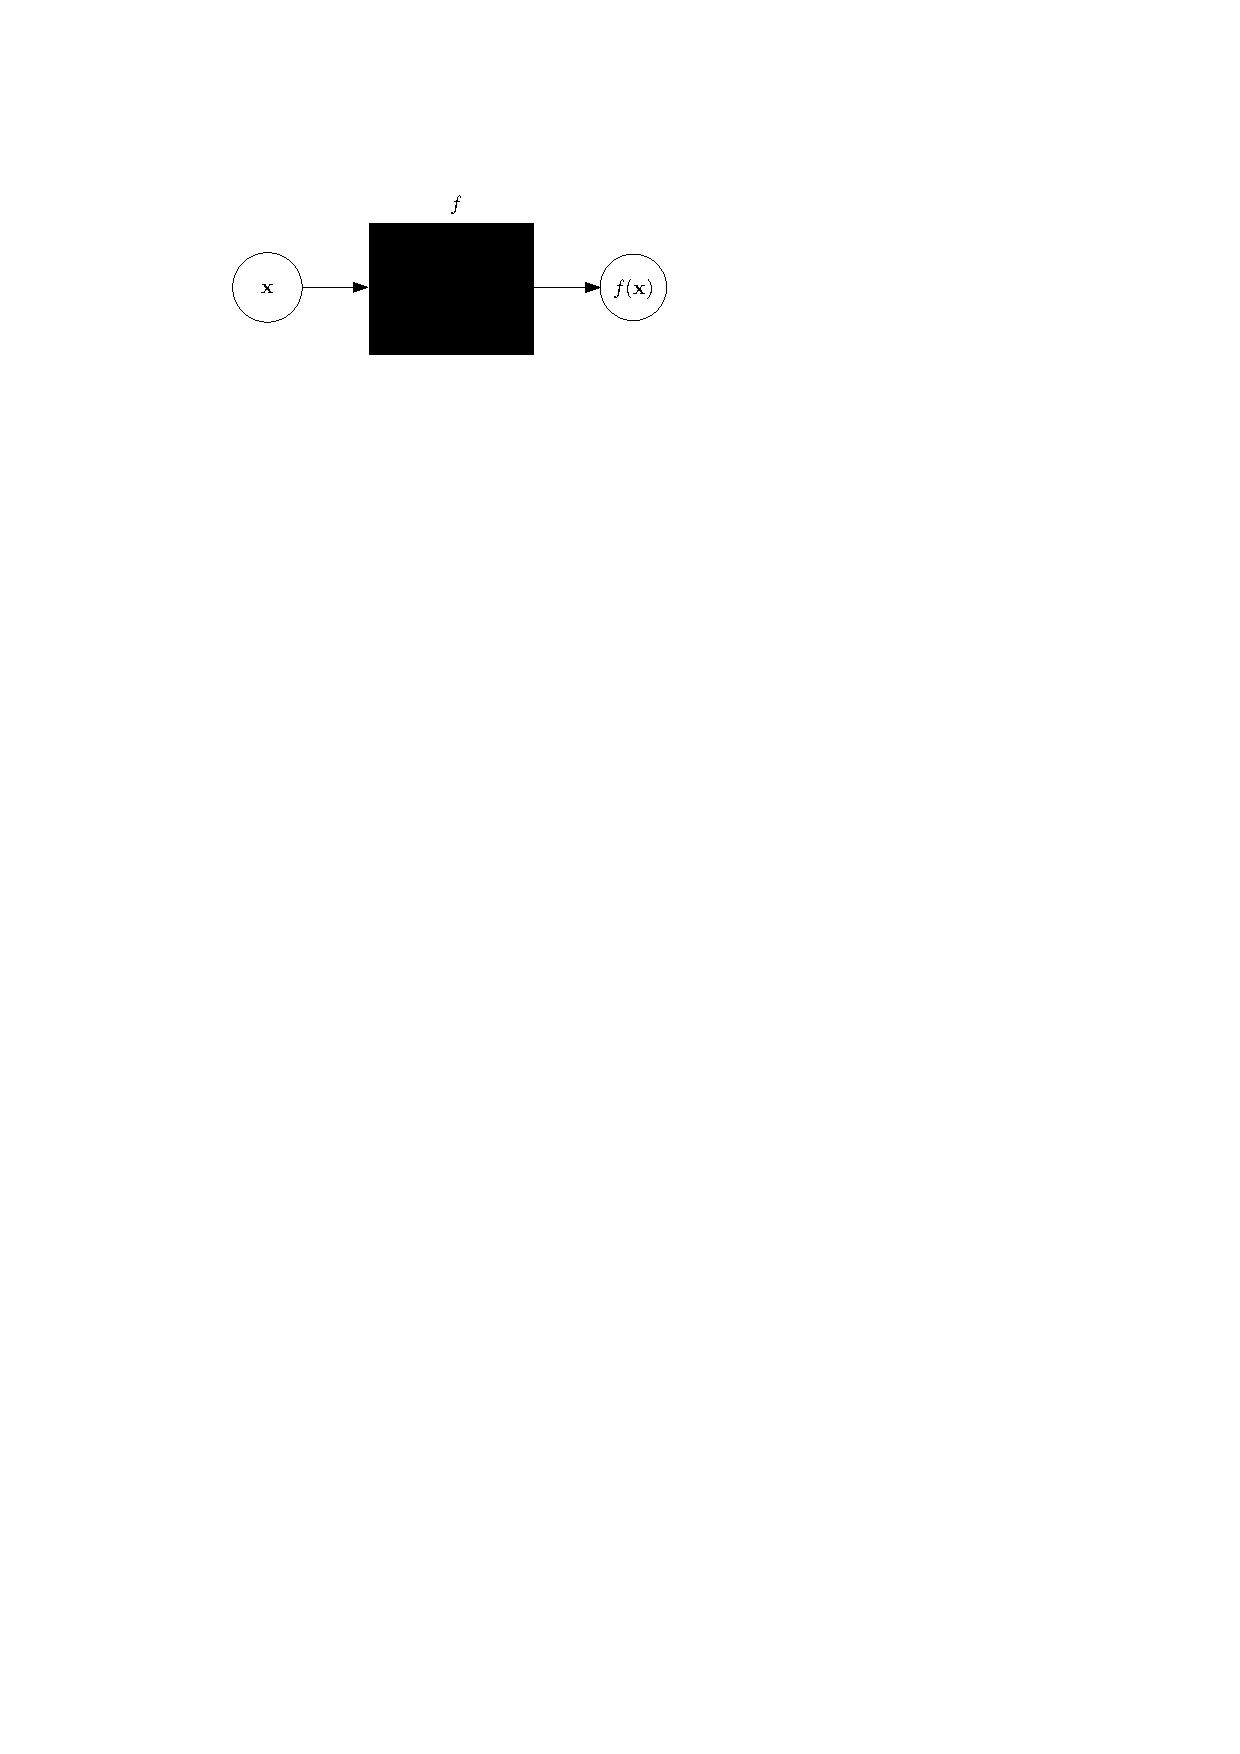
\includegraphics[width=0.4\linewidth]{img/black-box-function}
      % \caption{}
      \end{figure}
    \item in continuous domain: $\xx \in \mathbb{R}^D$
    \item only evaluation of the function value, \\
      \alert{no derivatives} or gradients available
      \begin{figure}
      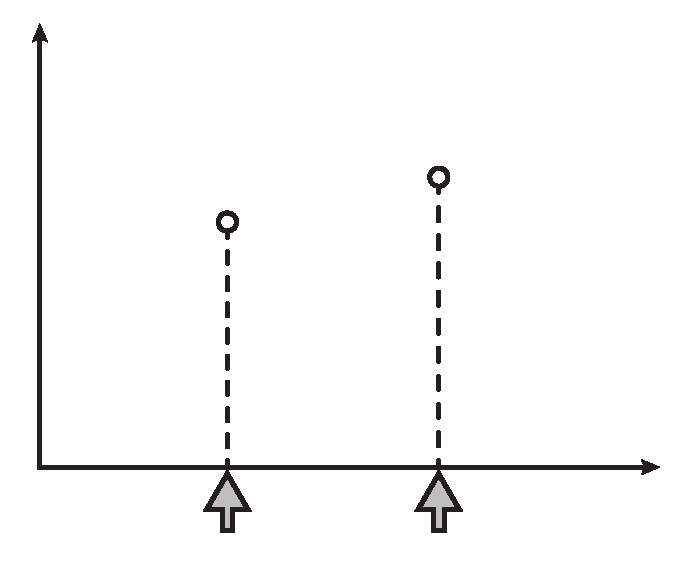
\includegraphics[width=0.4\linewidth]{img/black-box-samples}
      % \caption{}
      \end{figure}
  \end{itemize}
\end{frame}

\begin{frame}
  \frametitle{Optimization of expensive black-box functions}
  cost of the optimization:
  \begin{itemize}
    \item evaluations are \alert{expensive} and/or time-demanding
    \item \alert{search cost} $\sim$ the number of function evaluations
  \end{itemize}
  \vskip 2ex
  \pause
  \textbf{Goals}:
  \begin{itemize}
    \item find a solution $\xx$ with the smallest function \\
      value $f(\xx)$ as possible (WLOG, we consider \emph{minimization})
    \item \textbf{optimization} (minimization) is finding such $\xx^\star \in \mathbb{R}^D$ that
      \begin{displaymath}
        f(\xx^\star) = \min_{\forall \xx \in \mathbb{R}} f(\xx)
      \end{displaymath}
    \item use reasonable small number of function evaluations \\
      (the lower the better)
  \end{itemize}
\end{frame}

\begin{frame}
  \frametitle{EA's for expensive black-box optimization}
  \begin{itemize}
    \item EA's often manage to \alert{escape} from \alert{local optima}
    \item but usually use \alert{many} function \alert{evaluations}
  \end{itemize}
  \vskip 2ex
  \pause
  what can help:
  \begin{itemize}
    \item utilize already measured values \\
      (at least prevent measuring the same thing twice)
    \item learn the shape of the function landscape \\
      or learn the (global) gradient or step direction \& size
  \end{itemize}
\end{frame}

\subsection{Model-based methods}

\begin{frame}
  \frametitle{Model-based methods accelerating the convergence}
  several methods are used in order to decrease \\
    the number of objective function evaluations needed by EA's
  \vskip 2ex
  \begin{enumerate}
    \item Surrogate modelling
    \item Estimation of Distribution Algorithms (EDA's)
    \item Efficient Global Optimization (EGO)~\footfullcite{jones_efficient_1998}
  \end{enumerate}
\end{frame}

\begin{frame}
  \frametitle{Surrogate modelling}
  \textbf{Surrogate modelling}
  \begin{itemize}
    \item technique which builds an \alert{approximating model} \\
      of the fitness function landscape
    \item the model provides a \alert{cheap and fast} \\
      replacement of the fitness function
    \item evaluation of \blue{part} of the population/generations \\ with the \blue{original
      function} is necessary, but \alert{larger populations} or longer runs are possible
    \item generation of the points guided by EA \\
      (crossover, mutation,\ldots)
  \end{itemize}
\end{frame}

\begin{frame}
  \frametitle{Estimation of Distribution Algorithms (EDA)}
  \textbf{Estimation of Distribution Algorithms}
  \begin{itemize}
    \item the model represents a \alert{distribution} of solutions \\ in the \blue{input space}
    \item new candidate solutions are generated via \\ \alert{sampling the model}
    \item better solutions are selected for being represented \\ by the model in the next generation
  \end{itemize}
\end{frame}

\subsection{EGO}

\begin{frame}
  \frametitle{Efficient Global Optimization (EGO)}
  \begin{columns}[T]
  \column{5cm}
    \textbf{EGO} % \footfullcite{jones_efficient_1998}
    \begin{itemize}
      \item<1-> \textbf{needed}: specific kind of surrogate model which can express \alert{uncertainty of the prediction} in a new point
      \item<1-> EGO uses Kriging / Gaussian processes (GP)
      \item<2-> for any given input $\xx$\invisible<2>{, it gives a \alert{probability distribution} of the output value}
    \end{itemize}
  \column{5.5cm}
    \only<1>{
      \begin{figure}
      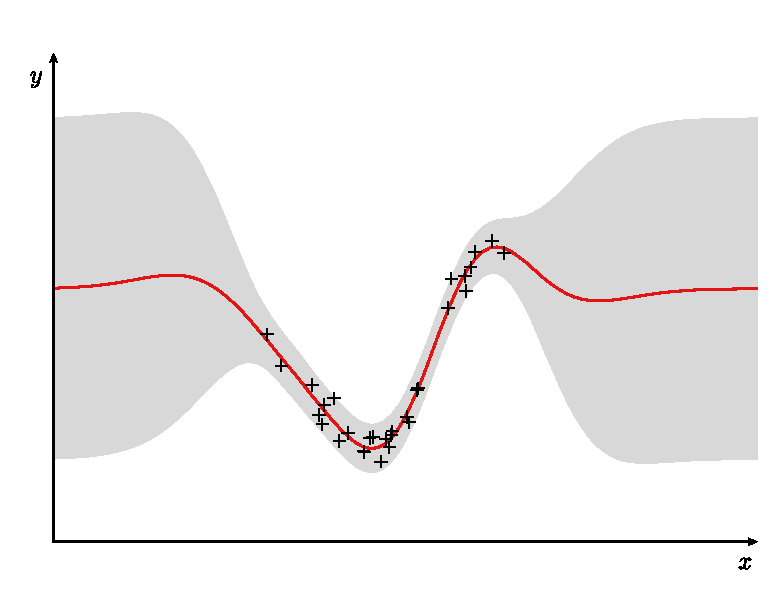
\includegraphics[width=\linewidth]{img/gp1}
      % \caption{}
      \end{figure}
    }
    \only<2>{
      \begin{figure}
      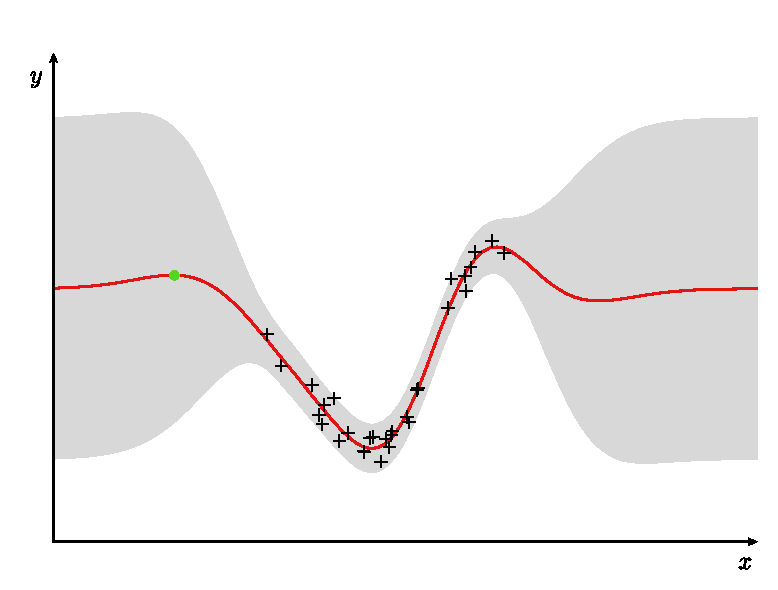
\includegraphics[width=\linewidth]{img/gp2-candidate}
      % \caption{}
      \end{figure}
    }
    \only<3>{
      \begin{figure}
      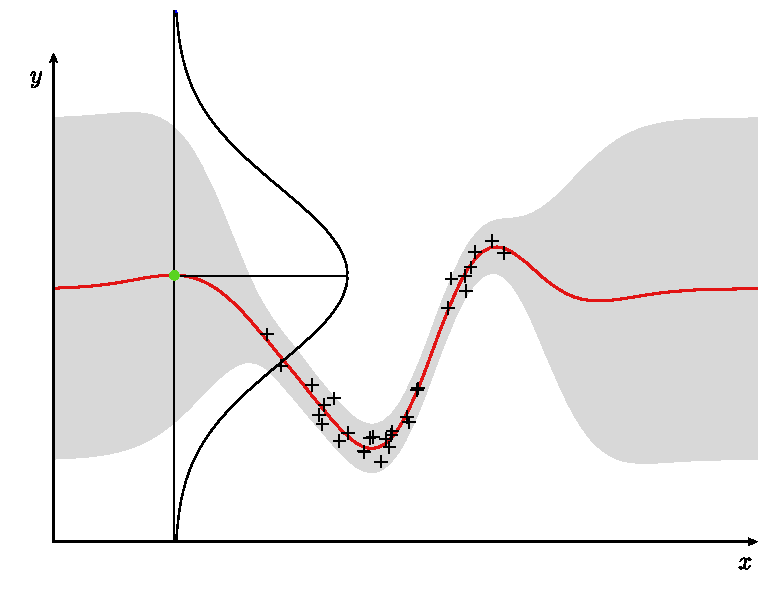
\includegraphics[width=\linewidth]{img/gp3-gauss}
      % \caption{}
      \end{figure}
    }
    \vskip 5cm
  \end{columns}
\end{frame}

\begin{frame}
  \frametitle{Efficient Global Optimization (EGO)}
  \begin{columns}[T]
  \column{5cm}
    \begin{itemize}
      \item the resulting output for a specified input $\xx$ is a 1-D Gaussian with
        \begin{itemize}
          \item \blue{mean} at the predicted value
          \item \blue{standard deviation} expressing uncertainty of this prediction
        \end{itemize}
    \end{itemize}
  \column{5.5cm}
    \only<1>{
      \begin{figure}
      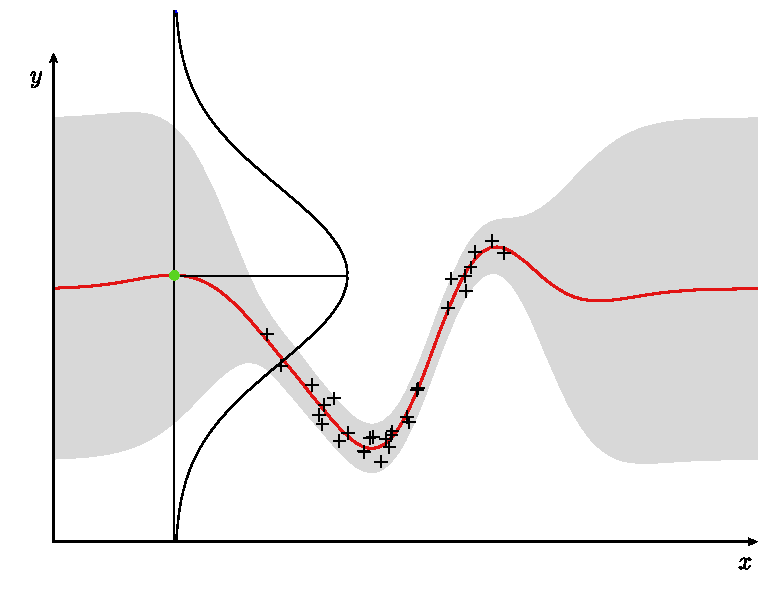
\includegraphics[width=\linewidth]{img/gp3-gauss}
      % \caption{}
      \end{figure}
    }
    \only<2->{
      \begin{figure}
      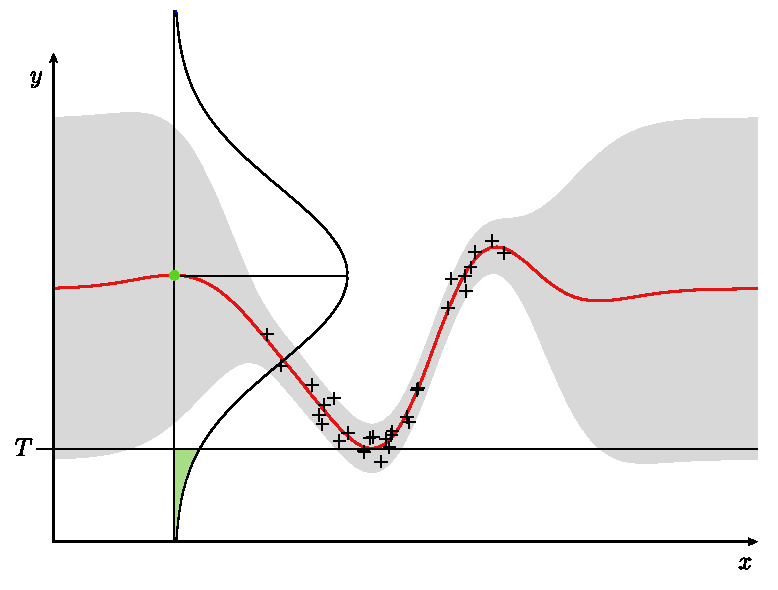
\includegraphics[width=\linewidth]{img/gp4-poi}
      % \caption{}
      \end{figure}
    }
  \end{columns}
  \begin{itemize}
    \item<2-> \alert{probability of improvement} ($\mathrm{PoI}$) is the probability that the function value will be lower than a specified \blue{target $T$}
      \begin{displaymath}
        \mathrm{PoI}_\blue{T}(\xx) = \Phi \left( \frac{\blue{T} - \hat{f}(\xx)}{\hat{\sigma}(\xx)} \right) = \mathrm{P}(\hat{f}(\xx) \leqq \blue{T})
      \end{displaymath}
  \end{itemize}
\end{frame}

\begin{frame}
  \frametitle{Efficient Global Optimization (EGO)}
  \textbf{EGO}
  \begin{enumerate}
    \item initialize random sample and build the GP model
    \item $\xx_\mathrm{max} \leftarrow$ maximize $\mathrm{PoI}(\xx)$
    \item evaluate found $\xx_\mathrm{max}$
    \item rebuild the GP model including the new data
    \item repeat from step 2
  \end{enumerate}
  \vskip 2ex
  maximizing the $\mathrm{PoI}$ is a way of \blue{balancing} between \alert{exploration} of the input space and \alert{exploitation} of the local optima
\end{frame}

%%%%%%%%%%%%%%%%%%%%%%%%%%%%%%%%%%
\section{MGSO}
%%%%%%%%%%%%%%%%%%%%%%%%%%%%%%%%%%

\begin{frame}
  \frametitle{Model Guided Sampling Optimization}
  \textbf{main idea}:
  \begin{itemize}
    \item consider the PoI to be a function proportional to a probability density
    \item sample this density to get a population of candidate solution
  \end{itemize}
  \textbf{motivation}: not getting trapped in local minima while exploring the search space
\end{frame}

\begin{frame}
  \frametitle{Model Guided Sampling Optimization}

  \textbf{MGSO}
  \begin{enumerate}
    \item generate a random initial sample and evaluate it resulting in a dataset $D$
    \item build a GP model $\hat{f}$ using $D$
    \item sample the PoI resulting in a new population $P$
    \item find the minimum $\xx_{\min} = \arg\min \hat{f}(\xx)$ of the GP and add to $P$
    \item evaluate all $\xx \in P$
    \item $D = D \cup P$
    \item repeat from 2
  \end{enumerate}
\end{frame}

%%%%%%%%%%%%%%%%%%%%%%%%%%%%%%%%%%
\subsection{Gaussian Processes}
%%%%%%%%%%%%%%%%%%%%%%%%%%%%%%%%%%

\begin{frame}
  \frametitle{Gaussian Process}
  \begin{itemize}
    \item GP is a stochastic approximation method based on Gaussian distributions
    \item let \newline
        $\XX = \{\xx_1, \dots, \xx_N\}$ \dots $N$ training data points
        $\yy = \{y_1, \dots, y_N \}, \quad y_i = f(\xx_i)\ $ \dots measured function values
    \item $\yy \in \R^N$ considered to be a realisation of a \blue{$N$-dimensional} Gaussian distribution
        with a covariance matrix $\CC$ and zero mean.
  \end{itemize}
\end{frame}

\begin{frame}
  \frametitle{Gausian Process covariance}
  \begin{itemize}
    \item covariance $\CC$ is given by \newline
        $\CC = \KK + \sigma^2 \II$ \newline
        $(\KK)_{ij} = cov(\xx_i, \xx_j) = \theta \exp(\frac{-1}{2\ell^2} (\xx_i - \xx_j)^\top (\xx_i - \xx_j)) $
    \item $\theta$ is the \blue{signal variance} and $\ell$ is the \blue{characteristic length scale} and $\sigma^2$
        is the \blue{signal noise}
  \end{itemize}
\end{frame}

\begin{frame}
  \frametitle{Gaussian Process prediction}
  \textbf{Making predictions}
  \begin{itemize}
    \item prediction $y^*$ in a new point $\xx^*$ is made by taking an $(N+1)$-dimensional
        Gaussian distribution with density \newline
        $p(\yy_{N+1} | \XX_{N+1})$
  \end{itemize}

  \begin{columns}[T]
  \column{5.5cm}
    \begin{itemize}
    \item since $\yy_N$ is known, we get a \alert{1D density} of $y^*$ by marginalization
        $$p(y^* | \XX_{N+1}, \yy_N)$$
        which is a 1D Gaussian distribution
    \end{itemize}
  \column{4.5cm}
    \begin{figure}
    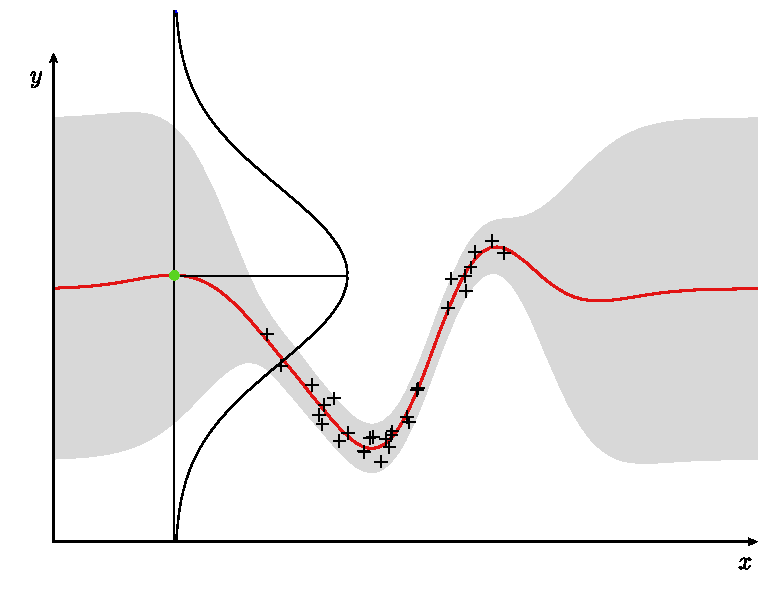
\includegraphics[width=\linewidth]{img/gp3-gauss}
    % \caption{}
    \end{figure}
  \end{columns}
\end{frame}

\subsection{Sampling PoI}

\begin{frame}
  \frametitle{Probability of improvement}
  \begin{columns}[T]
  \column{5cm}
    \begin{figure}
    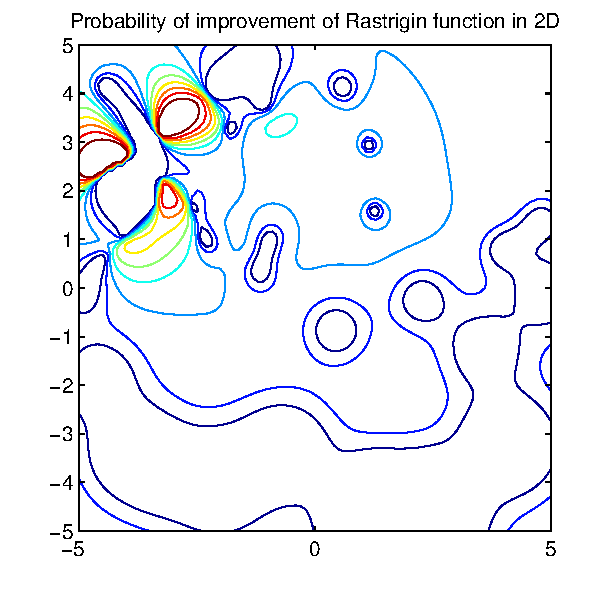
\includegraphics[width=\linewidth]{img/poi-example-color}
    % \caption{}
    \end{figure}
  \column{5.5cm}
    \begin{itemize}
      \item no explicit formula for $\mathrm{PoI}$
      \item improvement in a new point $\xx$ is probable when
        \begin{itemize}
          \item not many samples around, i.e. large $\sigma$ at $\xx$
          \item promising area is searched, i.e. low $f(\xx)$
        \end{itemize}
      \pause
      \item different way of generating new points
        \begin{itemize}
          \item \blue{EGO}: find the maximum of PoI
          \item \blue{MGSO}: sample the PoI as a distribution
        \end{itemize}
    \end{itemize}
  \end{columns}
\end{frame}

\begin{frame}
  \frametitle{Slice sampling}
  \begin{itemize}
    \item as no explicit formula for PoI exists, MCMC sampling methods are used
    \item Gibbs sampling (used in the article) showed to be very inefficient
    \item instead, \alert{slice sampling} used in the new version
  \end{itemize}
\end{frame}

\begin{frame}
  \frametitle{Slice sampling}
  \only<1>{
    \begin{figure}
    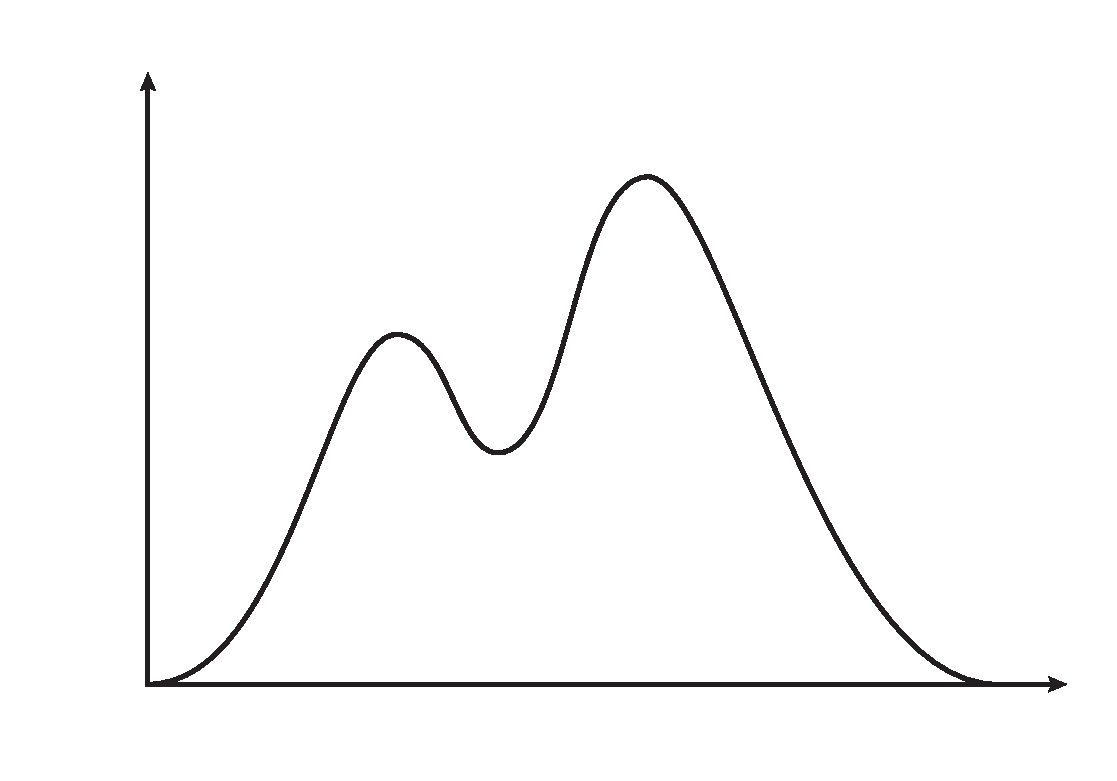
\includegraphics[width=0.6\linewidth]{img/slice-sampling-1}
    % \caption{}
    \end{figure}
  }
  \only<2>{
    \begin{figure}
    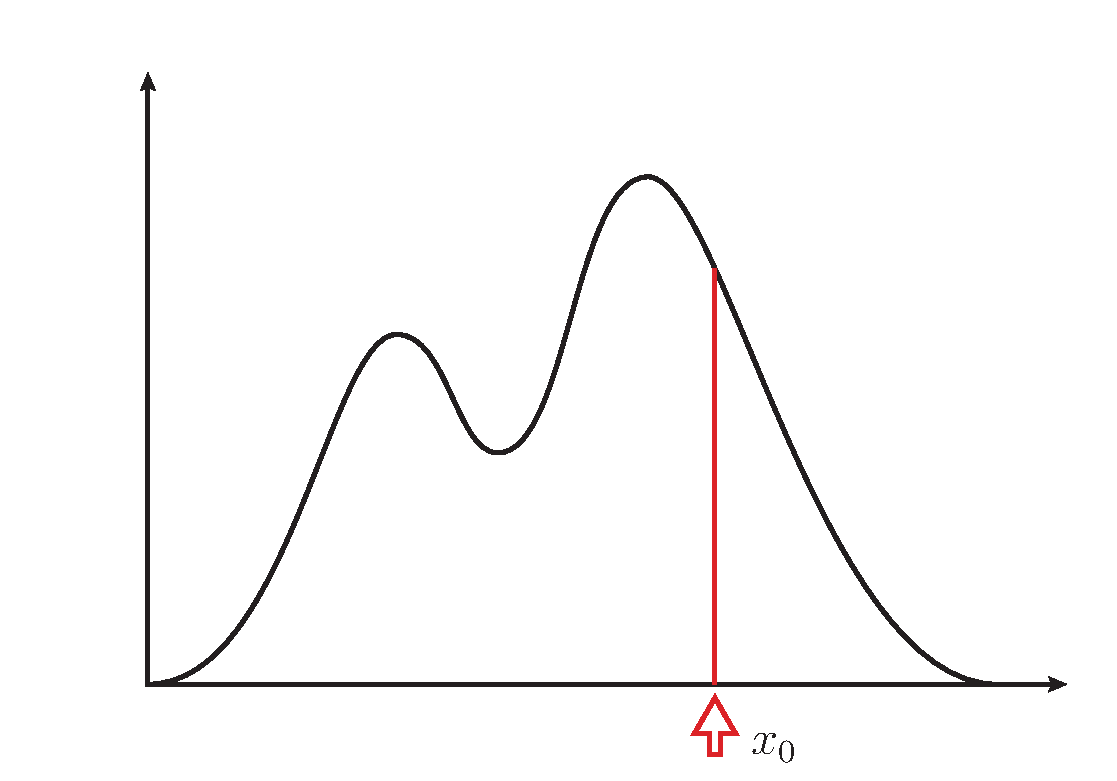
\includegraphics[width=0.6\linewidth]{img/slice-sampling-2}
    % \caption{}
    \end{figure}
  }
  \only<3>{
    \begin{figure}
    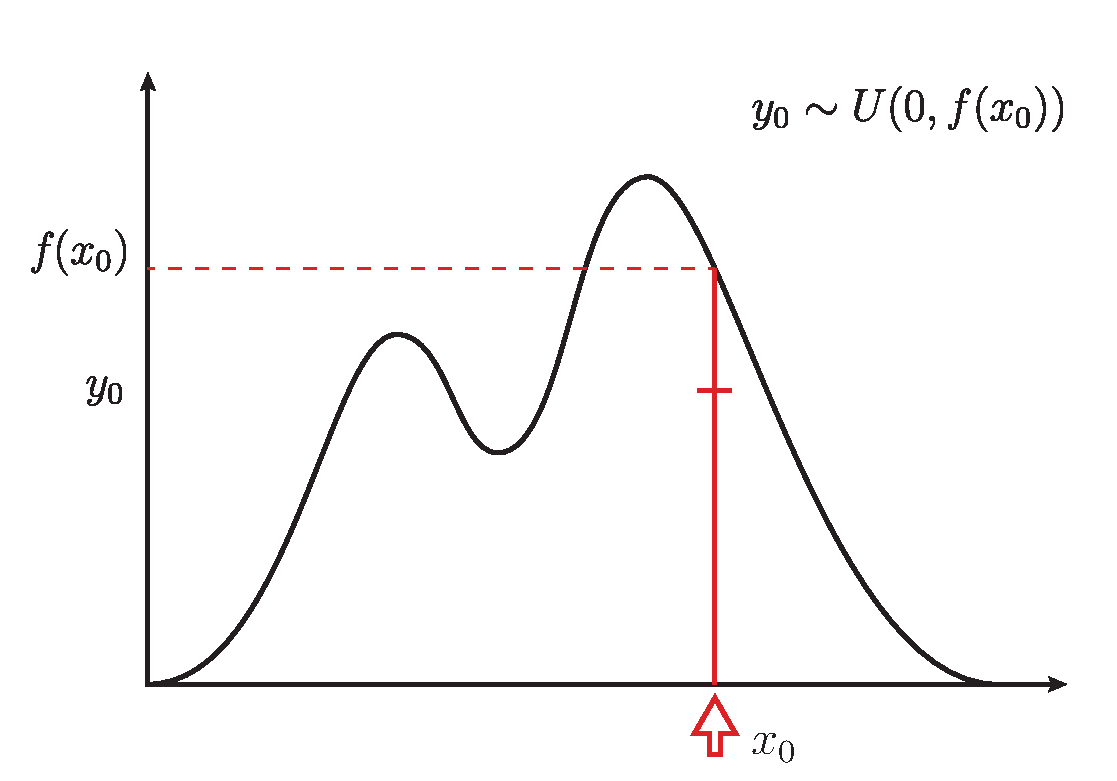
\includegraphics[width=0.6\linewidth]{img/slice-sampling-3}
    % \caption{}
    \end{figure}
  }
  \only<4>{
    \begin{figure}
    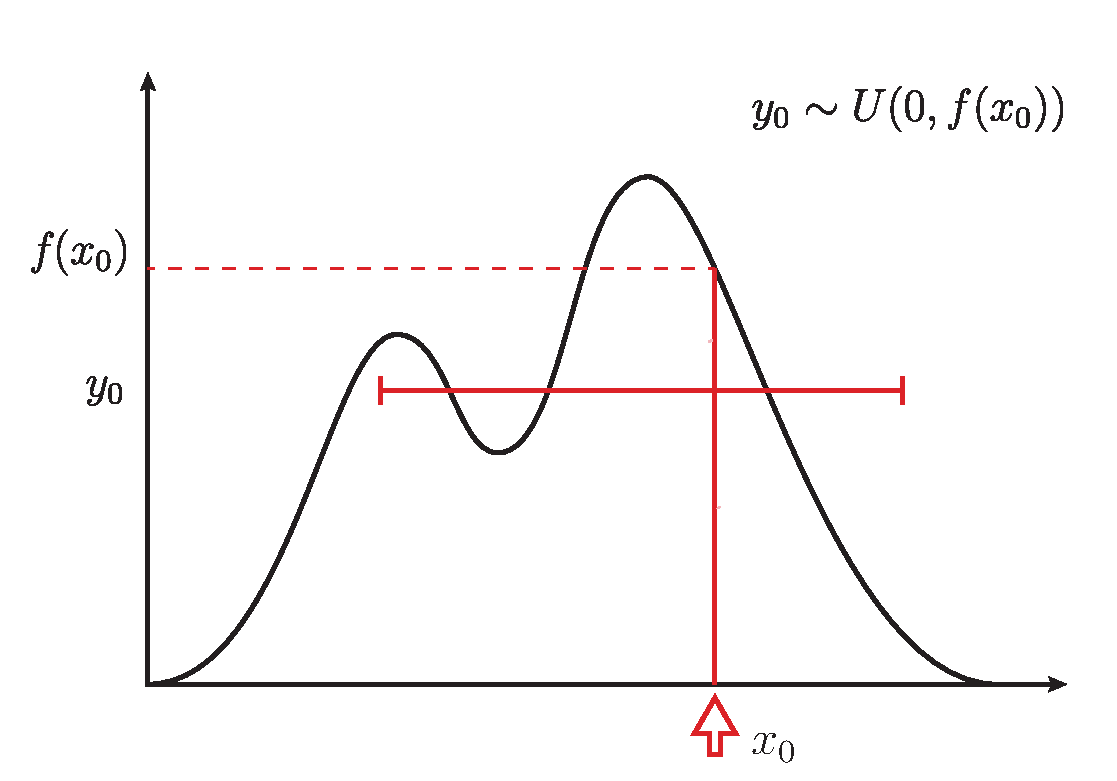
\includegraphics[width=0.6\linewidth]{img/slice-sampling-4}
    % \caption{}
    \end{figure}
  }
  \only<5>{
    \begin{figure}
    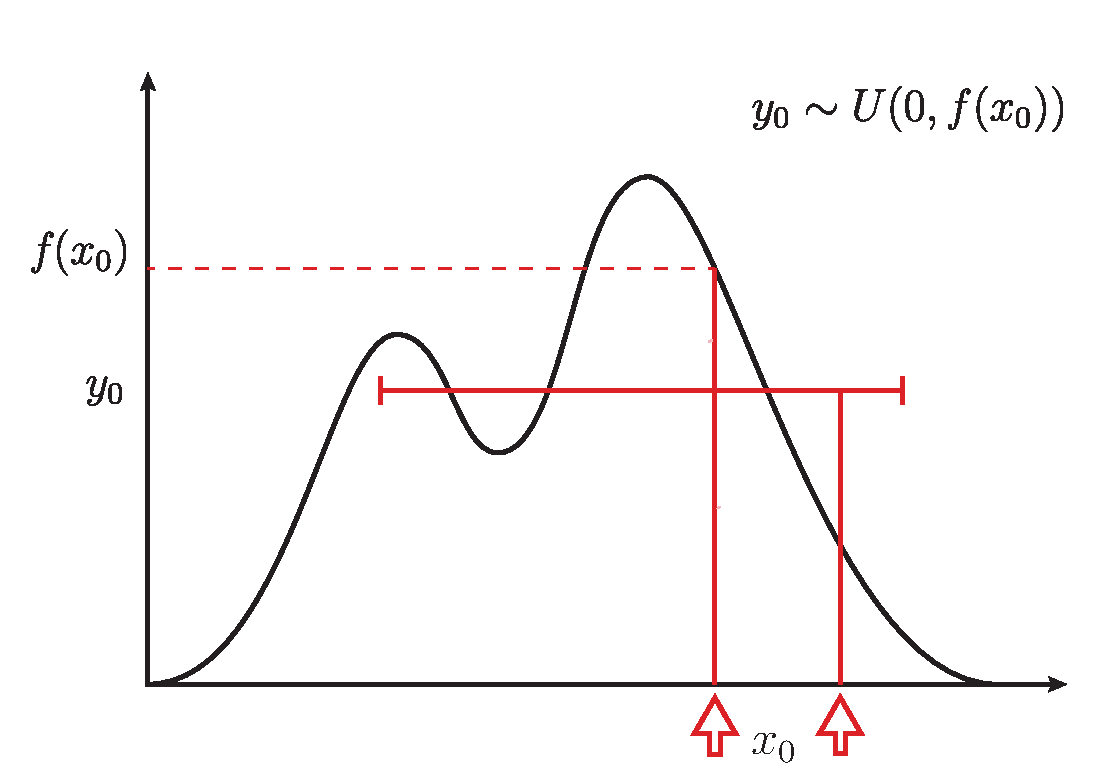
\includegraphics[width=0.6\linewidth]{img/slice-sampling-5}
    % \caption{}
    \end{figure}
  }
  \only<6>{
    \begin{figure}
    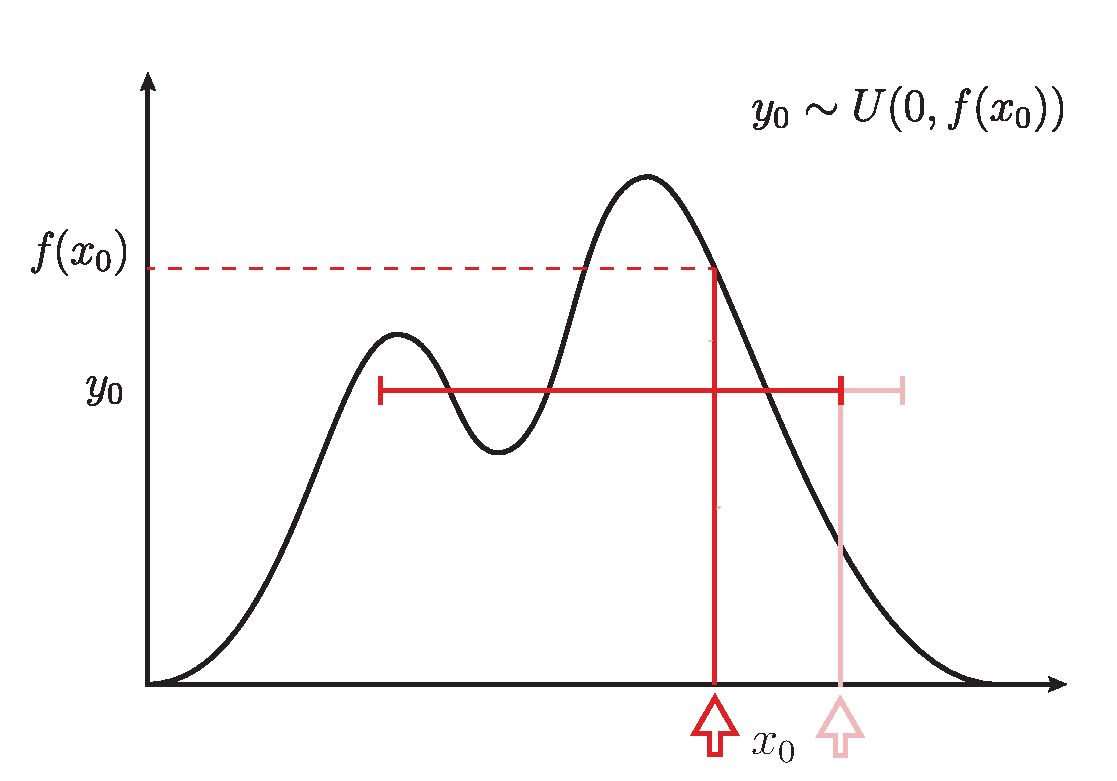
\includegraphics[width=0.6\linewidth]{img/slice-sampling-6}
    % \caption{}
    \end{figure}
  }
  \only<7>{
    \begin{figure}
    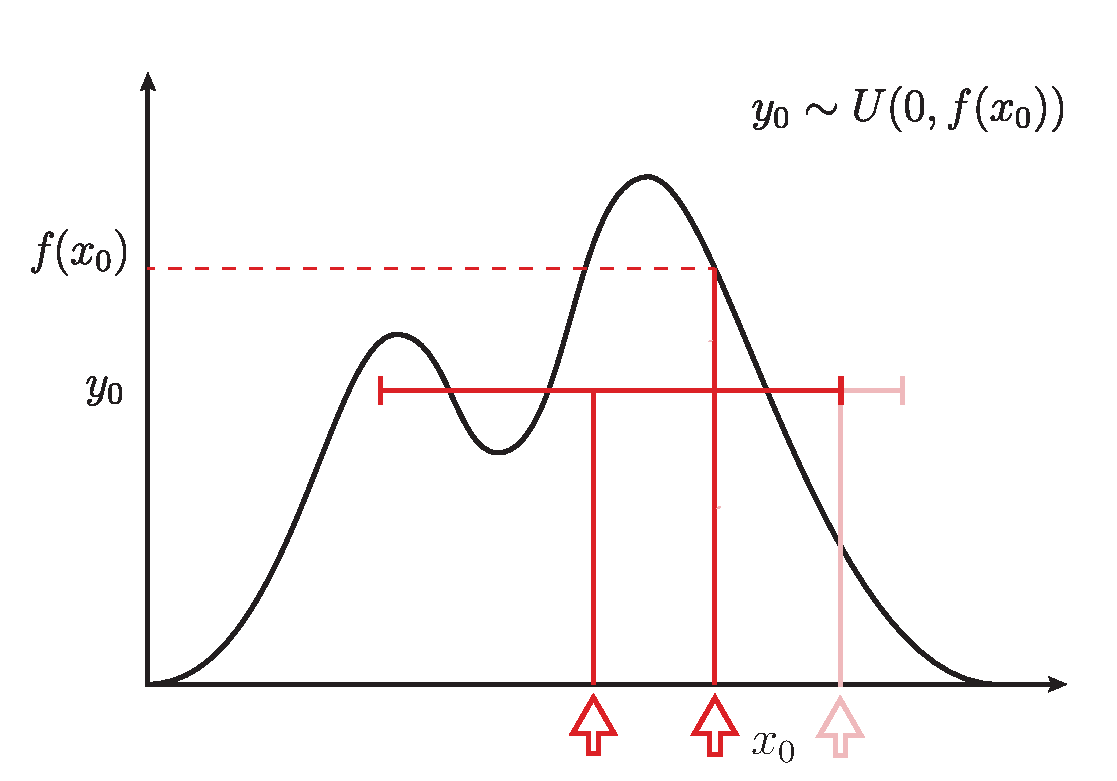
\includegraphics[width=0.6\linewidth]{img/slice-sampling-7}
    % \caption{}
    \end{figure}
  }
  \only<8>{
    \begin{figure}
    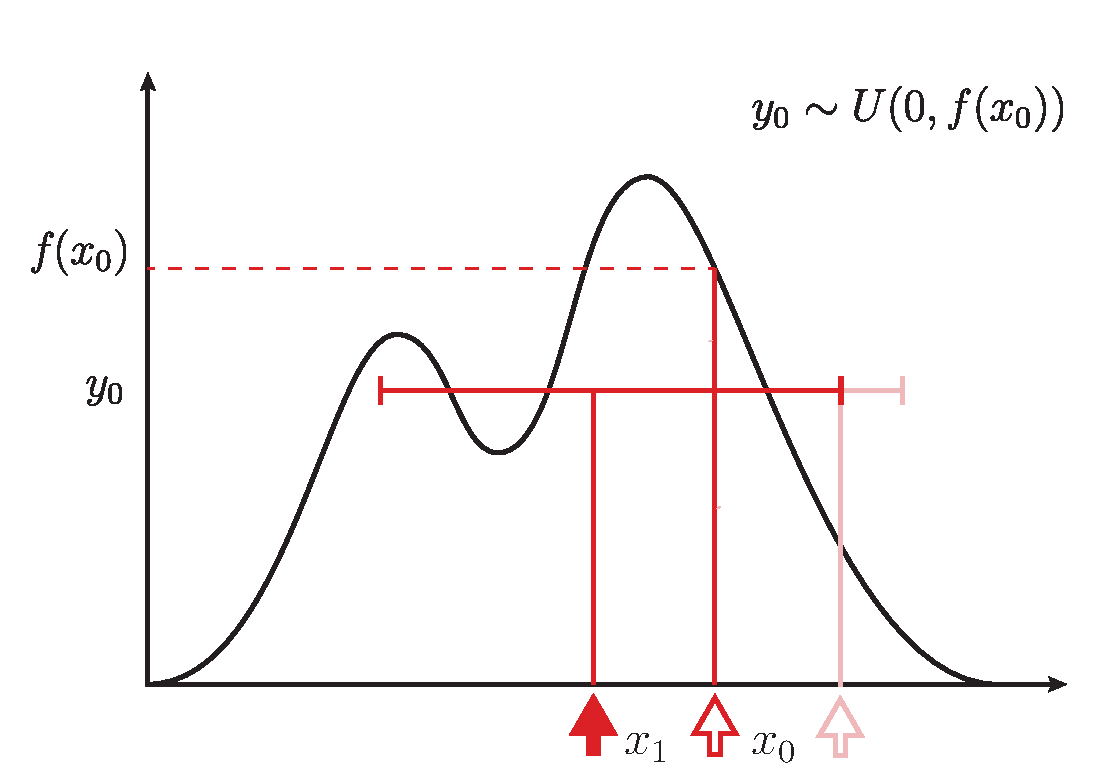
\includegraphics[width=0.6\linewidth]{img/slice-sampling-8}
    % \caption{}
    \end{figure}
  }
\end{frame}

\begin{frame}
  \frametitle{Implementation issues}
  \textbf{Numerical instability}
  \begin{columns}[T]
  \column{5cm}
    \begin{figure}
    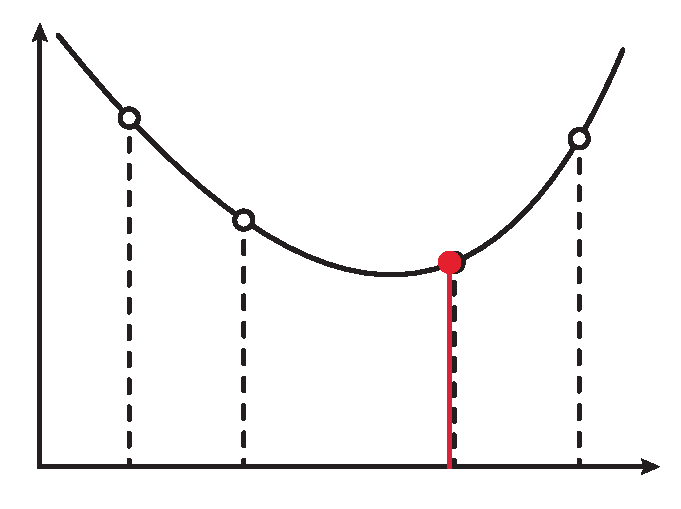
\includegraphics[width=\linewidth]{img/numerical-instability}
    % \caption{}
    \end{figure}
  \column{5.5cm}
    \begin{itemize}
      \item sampling a new point $(\xx', f(\xx'))$ close to one already in
          the dataset can cause numerical problems in covariance matrix inversion
      \item such points are rejected in sampling
    \end{itemize}
  \end{columns}
\end{frame}

\begin{frame}
  \frametitle{Implementation issues}
  \textbf{Degeneration of PoI}
  \begin{columns}[T]
  \column{5cm}
    \begin{figure}
    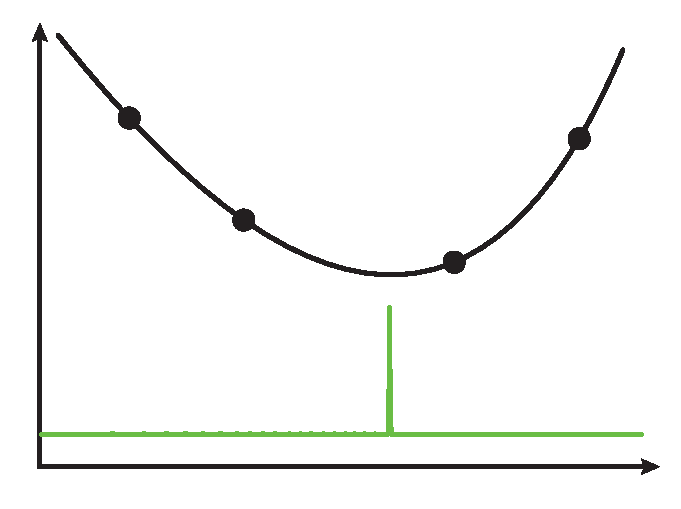
\includegraphics[width=\linewidth]{img/degenerate-poi}
    % \caption{}
    \end{figure}
  \column{5.5cm}
    \begin{itemize}
      \item PoI degenerates close to a discrete distribution in later phases of the optimization
      \item happens when the input space is well explored and the model's error estimate is low
      \item resolved by \alert{cropping} the input space to the region of the optimum and \alert{rescaling} to get
        better numerical resolution for sampling
    \end{itemize}
  \end{columns}
\end{frame}

\section{Preliminary results}

\begin{frame}
  \frametitle{Preliminary results}
  \begin{itemize}
    \item MGSO was tested on \blue{three benchmark} functions from BBOB testbed
      \begin{itemize}
        \item sphere
        \item Rosenbrock
        \item Rastrigin
      \end{itemize}
    \item three dimensionalities: 2D, 5D, 10D (not in LBA)
    \item compared to \blue{CMA-ES} (not in LBA)
  \end{itemize}
\end{frame}

\begin{frame}
  \frametitle{Results in 2-D}
  \begin{figure}
  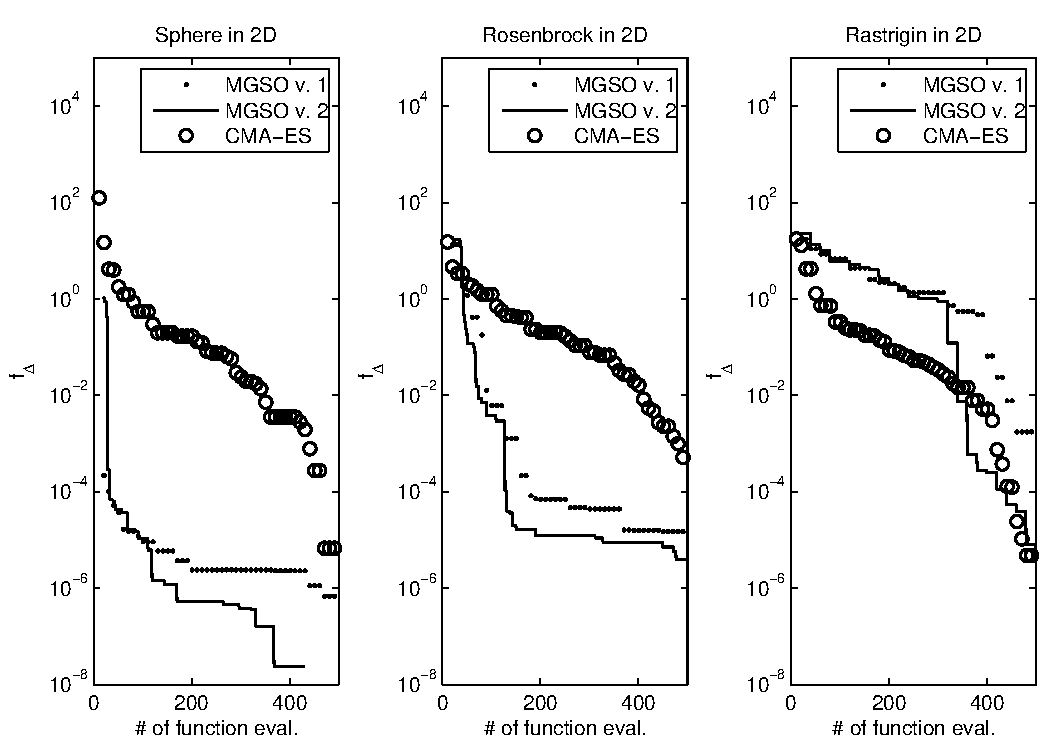
\includegraphics[width=0.7\linewidth]{img/optim_2D.pdf}
  % \caption{}
  \end{figure}
  {\small
    average results of the best-found fitness from 15 runs on different function instances }
\end{frame}

\begin{frame}
  \frametitle{Results in 5-D}
  \begin{figure}
  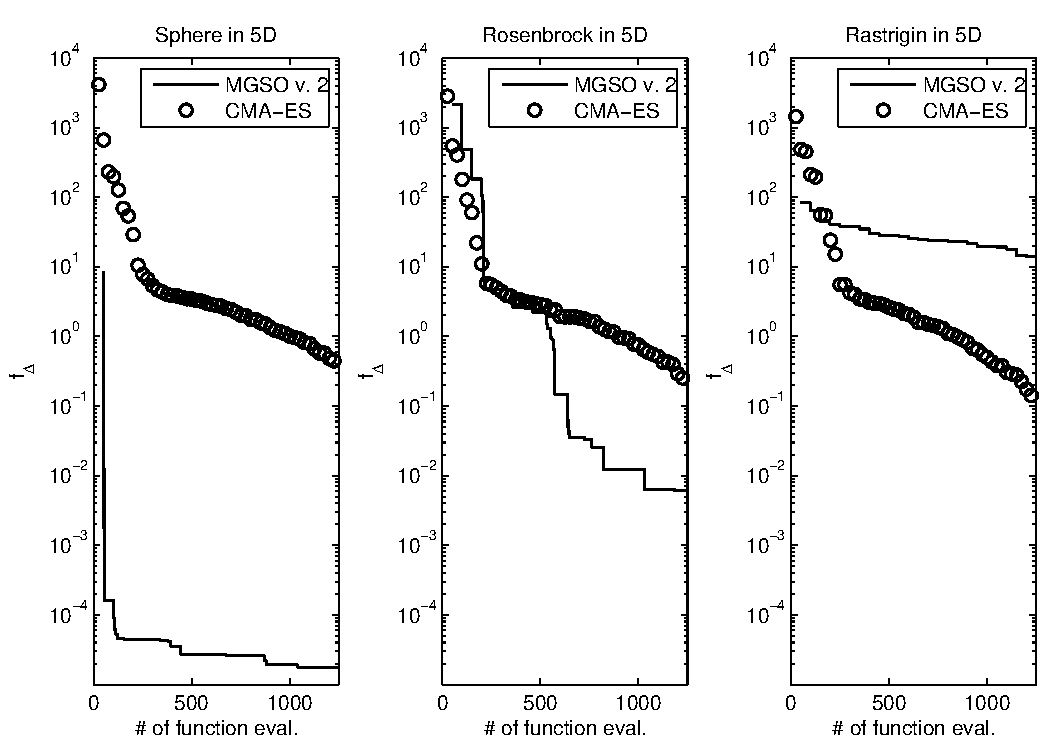
\includegraphics[width=0.7\linewidth]{img/optim_5D.pdf}
  % \caption{}
  \end{figure}
  {\small
    average results of the best-found fitness from 15 runs on different function instances }
\end{frame}

\begin{frame}
  \frametitle{Results in 10-D}
  \begin{figure}
  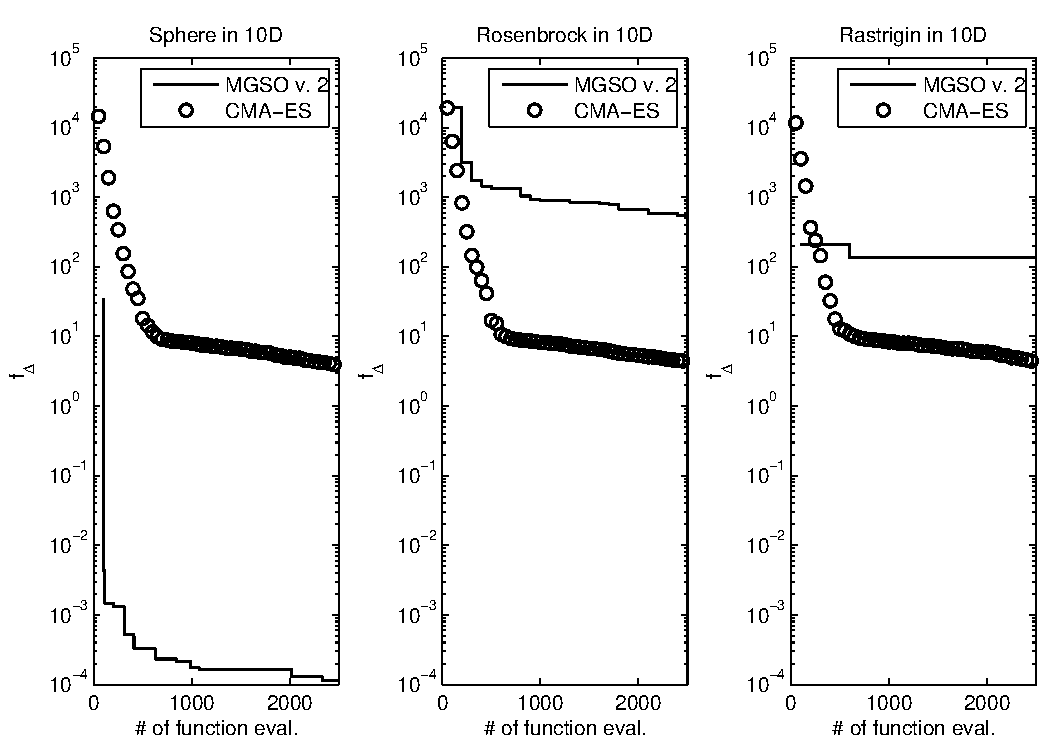
\includegraphics[width=0.7\linewidth]{img/optim_10D.pdf}
  % \caption{}
  \end{figure}
  {\small
    average results of the best-found fitness from 15 runs on different function instances }
\end{frame}

\begin{frame}
  \frametitle{Conclusion}
  \begin{itemize}
    \item MGSO showed to perform well on easy functions or in very low dimensions
    \item several issues have to be considered further
      \begin{itemize}
        \item better initial sampling
        \item model's hyperparameters training (GPML by Rasmussen)
        \item \uv{stronger finish}
      \end{itemize}
  \end{itemize}
\end{frame}

\begin{frame}
  \begin{center}
    {\Large Thank you! }
  \end{center}
\end{frame}

\end{document}
